\section{Analyse}
        
    
    \subsection{Kravliste}
        \begin{enumerate}
            \item Spillet skal være mellem 2 - 4 personer.
            \item Spillerne skal slå med en terningen på skift.
            \item Der skal udskrives en tekst, der omhandler det aktuelle felt, når spilleren lander på et felt.
            \item Spilleren skal købe feltet, hvis der landes på et frit felt.
            \item Spilleren skal betale husleje til ejeren, hvis der landes på et købt felt.
            \item Spilleren skal betale dobbelthusleje til ejeren, hvis der landes på en "par"-ejet hustand.
            \item Spillere modtager 2M, når start passeres.
            \item Spilleren ryger direkte i fængsel, hvis der landes på "GÅ I FÆNGSEL". Der modtages ikke 2M, hvis start passeres i forbindelse med dette.
            \item Sidder man i fængsel, bliver ens "Du løslades uden omkostninger"-kort brugt. Hvis kortet ikke haves betales der 1M.
            \item Landes der på "Chance", bliver effekten printet, og den printede effekt sker.
            \item Landes der på "Gratis parkering" sker ingenting, og turen går videre.
            \item Landes der på "På besøg" sker ingenting, og turen går videre.

            \item Spillerne starter med en balance på:
            \begin{enumerate}
                \item 16, hvis der er 4 spillere.
                \item 18, hvis der er 3 spillere.
                \item 20, hvis der er 2 spillere.
            \end{enumerate}
            %Efter de nye regler så starter spillerne med hhv. 20, 18 eller 16 Matadollars, alt efter om der er 2, 3 eller 4 spillere.
            \item Spillet slutter, når den første spiller har mistet alle sine penge.
            \item Spilleren med flest penge vinder, når spillet slutter vinder. Efterfølgende printes "Tillykke (spiller)", du har vundet!"

            %Efter de nye regler så er der når den første spille går bankerot
            \item Spillerne skal kunne gå flere omgange rundt på spillepladen.
            \item Spillet skal kunne køre på DTU’s databarer.

        \end{enumerate}

%---------------------------------------------------------------------------
%                             Input af usecases
%--------------------------------------------------------------------------
\input{UseCases.tex}

\pagebreak
\subsection{UseCase diagram}
    \begin{figure}[h]
        \advance\leftskip-3cm
        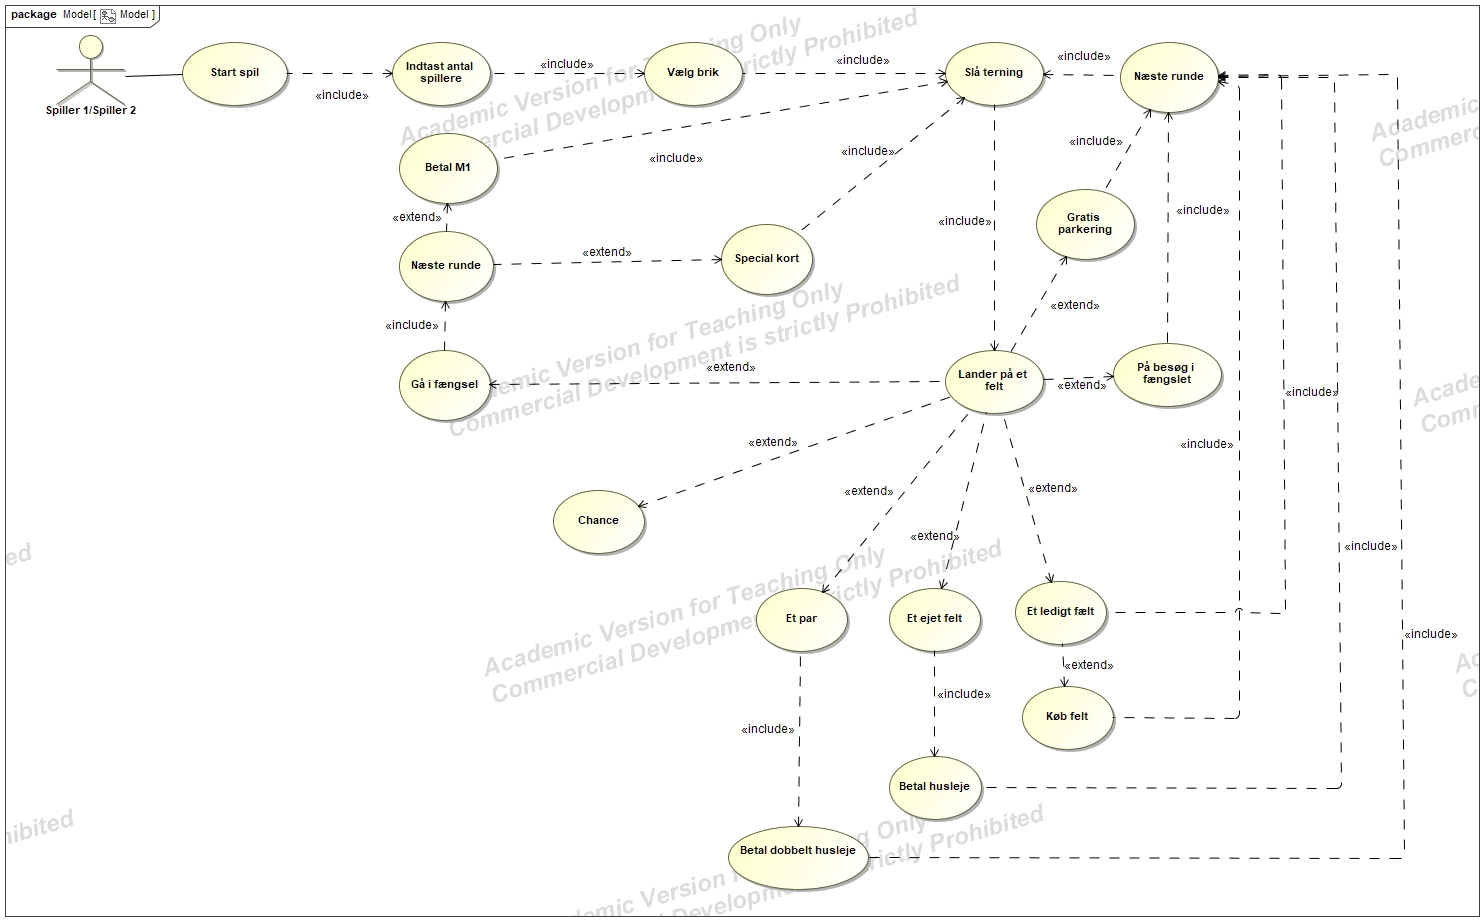
\includegraphics[width=20cm]{fig/UC-cdio3.jpg}
        \caption{UseCase diagram tegnet i MagicDraw}
    \end{figure}

\subsection{GRASP}
    GRASP står for \textit{General Responsibility Assignment Software Patterns}. GRASP bruges til at give det rigtige ansvar til de forskellige klasser, der bliver oprettet under udviklingen af et program. GRASP indeholder 9 patterns. Patterns bliver brugt til at strukturere et problem, samt at finde en passende løsning. De 9 patterns er:
        \begin{enumerate}
            \item Creator
            \item Information expert
            \item Low coupling
            \item Controller
            \item High cohesion
            \item Indirection
            \item Polymorphism
            \item Protected variations
            \item Pure fabrication
        \end{enumerate}
    (Der skrives mere når vi er nået længere i projektet)
